\chapter{Grundlagen \& Vorarbeiten}
\label{kapitel-grundlagen}
Im folgenden werden Begriffe aus dem Bereich Wissenmodellierung und Wissensrepräsentation näher erklärt, da diese die formale Grundlage der Arbeit bilden.

Dazu gehören Ontologien, für was sie stehen und die Beschreibung des OWL2 RL Fragments. Das Verständnis für einen Schlussfolgerer, sowie einige Hintergründe für die Umsetzungen von Ontologien in Datenbanken.

Außerdem werden auch einige Begriffe angesprochen die sonst für die Arbeit wichtig sind, aber nicht intuitiv zu erschließen sind. Dazu gehören unter anderem Regeln und Relationen.

\section{Ontologien}

Ontologien sind nach einem Formalismus erzeugte Beschreibungen eines Teilausschnittes der Welt, die formal ableitbare Aussagen ermöglichen. Sie haben damit eine entfernte Beziehung zu Datenbanken, die z.B. nach einem ER-Modell entwickelt wurden. Ontologien enthalten dabei die Struktur und Beziehung der Daten, sowie die Daten selbst. Anders als in einem ER-Modell sind aber die Daten und die Struktur nicht strikt von einander getrennt. Der Formalismus auf dem eine Ontologie aufsetzt ist im Rahmen der W3C Semantic Web Initiative stark von Logik geprägt. \cite{Hesse2002}

\subsection{Unterschied zu relationaler Datenbank}

Beim Abspeichern einer Ontologie in einer relationalen Datenbank sind zwei konzpetionelle Dinge zu beachten. In einer Ontologie gilt die \emph{unique name assumption}, das bedeutet das in der Ontologie verwendete Namen zum identifizieren von Entitäten eindeutig sind und sicher immer auf die selbe Entität beziehen. In OWL gilt das nur zum Teil, da es hier möglich ist auszudrücken, das zwei Namen identisch oder verschieden sind\cite{OWL1}\footnote{Die Ausdrücke sind \texttt{owl:sameAs} und \texttt{owl:differentFrom}.}. In einer Relation ist das nicht zwingend vorausgesetzt. Nur wenn Spalten als Schlüssel oder als \emph{unique} deklariert werden, wird sichergestellt das Namen eindeutig sind.
Der zweite Unterschied besteht darin, wie man über die Daten schließt. In einer Datenbank geht man davon aus, das man die komplette Welt modelliert hat und alle Fakten vorhanden sind. Kann etwas nicht gefunden werden, ist es nicht Teil des Modells und damit falsch. In einer Ontologie werden Fakten, die nicht vorhanden sind als unbekannt eingestuft. Sie sind damit weder wahr noch falsch. Datenbanken verwenden damit eine sog. \emph{closed-world assumption} (CWA) und Ontologien eine \emph{open-world assumption} (OWA).

\section{OWL2}
\label{abschnitt-owl2}

\begin{figure}[htb]
	\caption{Adaption des W3 Layercake\cite{W3SWLayerCake}}
	\label{image-w3-layercake}
	\begin{center}
	\scalebox{0.35}{
		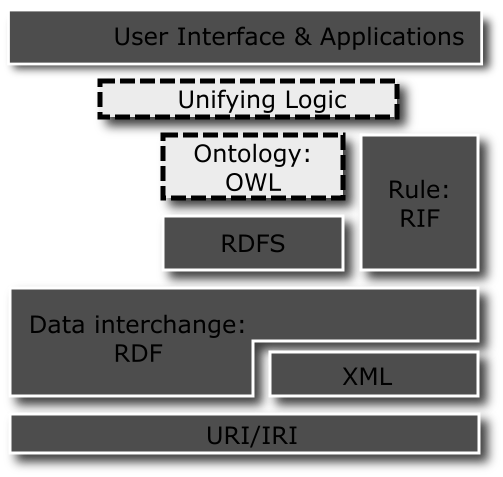
\includegraphics{images/w3-layercake.pdf}
	}
	\end{center}
\end{figure}


Abbildung \ref{image-w3-layercake} zeigt eine Adaption des offizielen W3 OWL Layercake\cite{W3SWLayerCake}. Es wurden alle Teile entfernt, die die Implementierung nicht betreffen. Dabei ist der helle Teil mit einer getrichelten Linie der in der Arbeit verwendete Teil. Der obere Teil ``User Interface \& Applications'' ist die Anwendungsschnittstelle, die z.B. durch die OWLAPI gekapselt wird. Die unteren Blöcke sind Web-Standards auf denen denen aufgebaut wird. Sie spielen in der Arbeit keine Rolle und sind für das Verständnis nicht näher benötigt.Der RIF Abschnitt ist hier erwähnt, weil er eine alternative Regelumsetzung bietet. Dies wird in Abschnitt \ref{abschnitt-rif} näher erläutert.

\begin{figure}[htb]
	\caption{Sprachkomplexitäten}
	\label{image-sprachhierarchie}
	\begin{center}
		\scalebox{0.4}{
			\includegraphics{images/sprachhierarchie.pdf}
		}
	\end{center}
\end{figure}

Die Abbildung \ref{image-sprachhierarchie} gibt einen Einblick in die Verhältnisse der Ausdrucksmächtigkeit, von OWL und wie sie in den größeren Kontext von Logik eingeordnet werden.

\begin{verbatim}
OWL2 TEXT
\end{verbatim}


\section{Sprachkomplexitäten}
Im folgenden werden verschieden Sprachen an Hand ihrer Komplexität kurz gegenüber gestellt, um einen Vergleichsbasis zu haben.

\begin{figure}[htb]
	\caption{OWL Logikeinordnungen, nach einer Vorlage aus \cite{OWLimLayerMap}}
	\label{image-owl-layer-map}
	\begin{center}
	\scalebox{0.35}{
		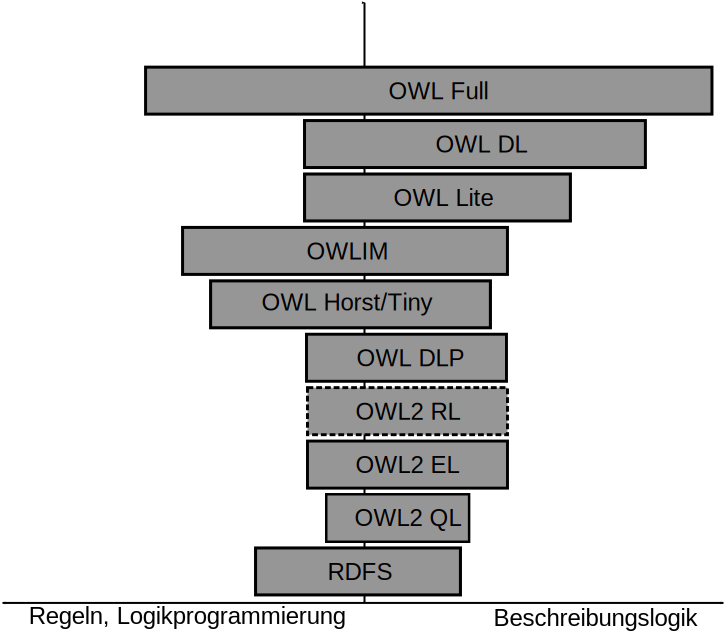
\includegraphics{images/owl-layer-map.pdf}
	}
	\end{center}
\end{figure}
Abbildung \ref{image-owl-layer-map} frei nach der Vorlage aus der OWLim Dokumentation. In dieser Abbildung wird der Einfluss der verschiedenen Semantiken von Logiken dargestellt.

\subsection{Attributive Language}
Die \emph{Attributive Language} ist eine einfache Beschreibungssprache. Sie wird mit $\mathcal{AL}$ abgekürzt und enthält folgende Operatoren für ihre Ausdrucksmöglichkeiten. Sie ist die Grundlage viler Sprachen, wie auch von OWL2.

$\mathcal{AL}$: C,D $\Longrightarrow$ A | $\top$ | $\bot$ | $\lnot$A | C $\land$ D | $\forall$r.C | $\exists$r

Diese attributive language kann durch weitere Operatoren in ihrere Ausdrucksmächtigkeit vergrößert werden. Für die Menge an Möglichkeiten hat sich dabei ein Namensschema herauskristallisiert. Dies ist zwar kein offizielles und eindeutiges Schema, wird aber von vielen Programmen wie z.B. Protégé verwendet.

Bei diesem Namenschema werden an die Buchstaben $\mathcal{AL}$ noch weitere Kürzel angehängt, die für die zusätzlichen Operatoren stehen.
\begin{itemize}
  \item $\mathcal{C}$ für volle Negation (Complement)
  \item (D) für konkrete Domänen\newline
Damit ist der Einsatz von Literalen möglich, z.B. in \emph{datatype properties}, \emph{data values} oder \emph{data types}.
  \item $\mathcal{U}$ Konzeptvereinigung (Union)
  \item $\mathcal{E}$ Existenzquantoren für komplexe Ausdrücke (Exists)\newline
Existenzquantoren sind für alle Arten von Ausdrücken erlaubt.
  \item $\mathcal{N}$ Kardinalitätseinschränkungen
  \item $\mathcal{I}$ Inverse Eigenschaften (Inverse)
  \item $\mathcal{O}$ Aufzählungen von \emph{object values} (Nominals)
  \item $\mathcal{H}$ Hierarchie von Eigenschaften (Role hierarchy)
  \item $\mathcal{F}$ Funktionale Eigenschaften
  \item $\mathcal{S}$ Die Abkürzung für $\mathcal{ALC}$ mit transitiven Eigenschaften
\end{itemize}
\cite{wiki:DescriptionLogic}

\subsection{Komplexität in Form der attributive language}
\begin{itemize}
  \item U2R2 basiert auf der DLP Sprache und ist damit ein Reasoner auf der $\mathcal{ALCHIF}$-Sprache ($\mathcal{SHIF}$). Hier gibt es allerdings Einschränkungen ähnlich wie in OWL2 RL. Es sind nicht, alle Konsturkte an jeder Stelle erlaubt, ansonsten sind Schlussfolgerungen nicht mehr vollständig.
  \item OWL2 basiert auf $\mathcal{ALCROIQ}$ ($\mathcal{SROIQ}$) \cite{Krötzsch2008}
\end{itemize}


\begin{figure}[htb]
	\caption{Sprachkomplexitäten}
	\label{image-sprachkomplexitaeten}
	\begin{center}
		\scalebox{0.4}{
			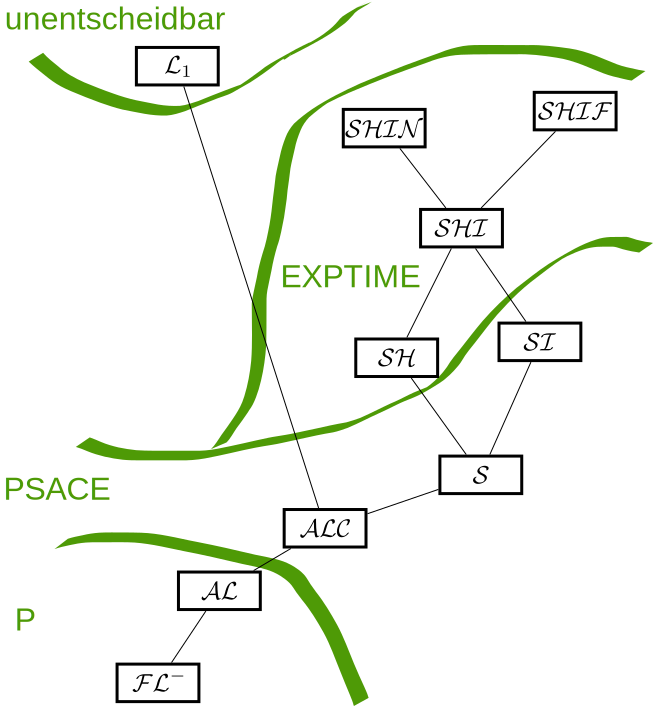
\includegraphics{images/sprachkomplexitaeten-wimo-blatt4.pdf}
		}
	\end{center}
\end{figure}
Die Abbildung \ref{image-sprachkomplexitaeten} ist frei nach der Vorlesung/Übung Wissensmodellierung \cite{vonHenke2009} modelliert. Es wird das ``computational cliff'' dargestellt. Man kann erkennen welche Sprachen welche Berechnungskomplexitäten haben

\begin{table}
	\caption{Sprachkomplexitäten}
	\label{table-sprachkomplexitaeten}
%	\rowcolors{3}{white}{lightgray}
	
	\scalebox{0.74}{
		\renewcommand{\arraystretch}{1.2}
		\begin{tabular}{|M{2cm}|p{2cm}|p{3cm}|p{3cm}|p{3cm}|p{3cm}|}
		\hline
		\rr Sprache & \rr Schluss\-folger\-ungs\-problem & \rr Komplexität der Taxonmie & \rr Daten\-komplexität & \rr Abfrage Komplexität & \rr Kombinierte Komplexität \tn
		\hline
		\hline
		\multirow{3}{*}{OWL-DL} & Ableitung & NEXPTIME-vollständig & Offen & Nicht anwendbar & NEXPTIME-vollständig \\ 
		\cline{2-6}
								& Abfragen & Offen & Offen & Offen & Offen \\
		\hline
		\multirow{3}{*}{DLP} & Ableitung & In EXPTIME & PTIME-vollständig & Nicht anwendbar & In EXPTIME \\
							\cline{2-6}
							& Abfragen & In EXPTIME & PTIME-vollständig & In EXPTIME & In EXPTIME \\
		\hline
		\rr \multirow{4}{2cm}{OWL2 Direct Semantics} & Ableitung & 2NEXPTIME-vollständig & entscheidbar, aber Komplexität offen & Nicht anwendbar & 2NEXPTIME \\
			\cline{2-6}
			& Abfragen & Entscheidbarkeit offen & Entscheidbarkeit offen & Entscheidbarkeit offen & Entscheidbarkeit offen \\
		\hline
		\multirow{3}{*}{OWL2 EL} & Ableitung & PTIME-vollständig & PTIME-vollständig & Nicht anwendbar & PTIME-vollständig \\
			\cline{2-6}
			& Abfragen & PTIME-vollständig & PTIME-vollständig & NP-vollständig & PSPACE-vollständig \\
		\hline
		\multirow{3}{*}{OWL2 QL} & Ableitung & NLogSpace-vollständig & In AC$^0$ & Nicht anwendbar & NLogSpace-vollständig \\
			\cline{2-6}
			& Abfragen & NLogSpace-vollständig & In AC$^0$ & NP-vollständig & NP-vollständig \\
		\hline
		\multirow{2}{*}{OWL2 RL} & Ableitung & PTIME-vollständig & PTIME-vollständig & Nicht anwendbar & PTIME-vollständig \\
			\cline{2-6}
			& Abfragen & PTIME-vollständig & PTIME-vollständig & NP-vollständig & NP-vollständig \\
		\hline
		\end{tabular}
	}
	\cite{WebontTractable}
	\cite{OWL2Complexities}
	\cite{ComplexityNavigator}
\end{table}

\section{Kriterien der Wissensrepräsentation}

Die Wissensrepräsentation ist zentraler Bestandteil eines KI-Systems. Eine Wissensrepräsentation wird zu jedem Bereich von intelligenten rechnergestützten Systemen benötigt.

Ein Wissensrepräsentationsformalismus kann für verschiedene Anwendungsgebiete ausgelegt sein, daher gibt es einige allgemeine Kriterien, um solche Sprachen einzuordnen.

Die wichtigsten Begriffe zur Einordnung dabei sind:
\begin{itemize}
	\item \textbf{Korrektheit}:
Ein Verfahren ist korrekt, wenn es nicht möglich ist falsche Schlüsse aus einer Wissenrepräsentation zu ziehen.
	\item \textbf{Vollständigkeit}:
Ein Verfahren ist vollständig, wenn alle korrekten Schlüsse folgerbar sind.
	\item \textbf{Entscheidbarkeit}:
Ein Verfahren ist entscheidbar, wenn ein Algorithmus für das Schlussfolgern existiert.
	\item \textbf{Komplexität}:
Die Komplexität beschreibt den theoretischen \emph{worst-case} Aufwand für den Schlussfolgerungs-Alogrithmus
\end{itemize}

\section{OWL2 RL Eigenschaften}
Das OWL2 RL Sprachfragment wurde speziell für Anwendungsgebiete entwickelt, die die größtmögliche Ausdrucksmächtigkeit benötigen, ohne dabei die Eigenschaft verlieren zu wollen effizient ableitbar zu sein. Effizient ist dabei im theoretischen Sinne zu verstehen, d.h. die Ableitungsfunktion ist in polynomieller Zeit ausführbar. Die Sprachuntermenge von OWL2 wurde dabei so gewählt, dass sie günstig mit einem regelbasierten Ansatz abzuleiten ist. Dazu wurde auch direkt Inferenzregeln angegeben, die diesem Fragment eine Semantik gibt. Der Entwurf dieses Sprachfragement wurde dabei von DLP \cite{Grosof2003} und pD* \cite{Li2006} inspiriert.

Damit fällt OWL2 RL auch in die Kategorie der monotonen Sprachen, das bedeutet wenn neue expliziten Fakten zur Wissensbasis hinzugefügt werden, dann fügen diese zwar durch Ableitung neue implizite Fakten zur Wissensbasis hinzu, aber unter keine Umständen können die expliziten Fakten das Entfernen von bereits abgeleiten Fakten verursachen. Damit kann das Hinzufügen von neuen Fakten die abgeleitete Wissenbasis nur monoton erweitern.

Um einige gewünschte Eigenschaften für die Sprache zu erhalten ist es dabei nötig nicht nur die verwendeten Konstrukte einzuschränken, sondern auch die Syntax. In OWL2 RL Profilbeschreibung wird eine Grammatik angegeben, an welcher Stelle welche Konstrukte verwendet werden dürfen.

Sofern sich eine Ontologie an die syntaktischen Rahmenbedigungen des Sprachfragments hält und ein Schlussfoglerer entsprechend der angebenen Regelsemantik implementiert ist, können sich daraus einige positive Kriterien ableiten lassen. So ist dann garantiert, das \emph{alle} und \emph{nur gültige} Ergebnisse vom Schlussfolgerer geliefert werden. Das Verfahren für die Wissensrepräsentation ist damit korrekt und vollständig (siehe Beweis in \cite{OWL2Profiles}).
Mit dieser regelbasierten Implementierung ist es sogar möglich in nicht-syntaktisch konformen Ontologien zu schlussfolgern. Es ist dann zwar nicht mehr möglich alle Ergebnisse zu ermitteln, aber es werden zumindest weiterhin nur gültige Ergebnisse abgeleitet.

Eine montone Logik ist besonders wichtig für den Einsatz im Web. Hier werden viele kleine verteilte Wissensbasen erzeugt. In einer Sammlung solcher Wissensbasen kann dann geschlussfolgert werden. Wird diese Sammlung erweitert, verkleinert oder verändert ist es natürlich umständlich, wenn wieder über alle anderen Beziehung geschloßen werden müsste. Durch eine montone Logik ist eine Umsetzung mit solchen Anforderungen besonders gut zu realisieren.


\subsection{RIF}
\label{abschnitt-rif}
RIF steht für Rule Interchange Format. Es ist ebenfalls ein Projekt des W3C \cite{RIF2005}. Ziel dabei ist es Schlussfolgerungsregeln in XML abzubilden. Damit können die Regeln ausgetauscht werden und regelbasierte Schlussfolgerer können für eine einheitliche Schnittstelle implementiert werden.

In der Spezifikation zu diesem Format gibt es auch eine Dokument darüber \cite{Reynolds2009}, wie die Regeln des OWL2 RL Fragments dargestellt werden können.

Dieser Ansatz kann allerdings in der Praxis noch nicht verwendet werden, da weder die RIF Spezifikation fertig ist, noch gibt es Schlussfolgerer und kaum Werkzeuge, die mit RIF umgehen können.


\subsection{Aufgabe eines Reasoner}
Allgemein muss ein Schlussfolgere die Frage beantworten, ob eine beliebige Formel $\Theta$ Modell der Ontologie $\Psi$ ist, kurz $\Theta \models \Psi$. Alle Anfragemöglichkeiten die ein Reasoner hat sind spezielle Formen solche Ergebnisse abzufragen.

Es lässt sich dabei in zwei Hauptaufgaben einteilen.
\begin{itemize}
  \item Klassifizierung
  \item Realisierung
\end{itemize}
Diese beiden Aufgaben sind der zentrale Dienst eine Schlussfoglerers. 

Die Klassifizierung soll die Struktur der Ontologie bestimmen, d.h. die Beziehung der Klassen bzw. Konzepte zueinander. Was sind die Unterklassen einer bestimmten Klasse oder welche Klassen sind äquivalent.
Die Realisierung bestimmt Beziehung zwischen Individuen. Welche Individuen sind Mitglieder von Klassen und über welche Beziehungen sind sie untereinander verbunden.

\section{Regeln}
Das OWL2 RL Profil wurde unter dem Aspekt entiwckelt, dass Inferenzen darin gut mit einem regelbasierten Ansatz umzusetzen sind.

Wie dabei die Umsetzung der Regeln in SQL stattfindet wird in entsprechenden Abschnitt \ref{abschnitt-regelbeispiele} näher erklärt. Hier wird vorab der Aufbau und die Bedeutung der in der OWL2 RL Spezifikation angegebenen Regeln näher gebracht.

Eine Regel setzt sich grundsätzlich aus zwei Dingen zusammen. Das ist zum einen die Vorbedingung und zum anderen die Nachbedingung\footnote{In den folgenden Tabellen, in denen Regeln beschrieben werden, wird die Vorbedingung mit \emph{if} abgekürzt und die Nachbedingung mit \emph{then}.}. Wenn für die Vorbedingung eine gültige Belegung in der Ontologie gefunden werden kann, dann gilt die Nachbedingung. Das Wort Belegung macht deutlich, das die Vorbedingung und Nachbedingung Variablen enthalten können. Variablen sind dadurch gekennzeichnet, das sie mit einem ``?'' vor ihrem Namen beginnen und kleingeschrieben sind.

Die Vorbedingung und Nachbedingung enthalten immer Tripel oder Listen. Tripel sind bekannt aus dem RDF-Bereich \cite{RDF2004}. Damit werden zwei Entitäten über das mittlere Element in Beziehung gesetzt. Das sieht z.B. so aus:
\begin{verbatim}
T('Walter', rdf:type, 'Person')
\end{verbatim}
Listen sind ein Konstrukt, um die Darstellung von Listen über die Tripels zu vereinfachen. Sie lassen sich aber auf Tripels zurückführen.

Eine komplette Regel kann foglendermaßen dagestellt werden:

\begin{table}[htb]
\begin{center}
\begin{tabular}{m{6cm}|m{4cm}}
if & then \\ \hline
T(?property, rdfs:domain, ?class),\newline
T(?x, ?property, ?class) & T(?x, rdf:type, ?class)
\end{tabular}
\end{center}
\caption{Die Regel prp-dom}
\label{rule-prp-dom}
\end{table}

Auf der Seite der Vorbedingung sind zwei Tripel, d.h. es muss für beide gleichzeitig eine Belegung der Variablen gefunden werden. Für jede gültige Belegung der Variablen gilt dann die Belegung der Variablen auf der rechten Seite.

\section{Delta-Relation}
Im späteren Verlauf wird häufiger auf Delts oder delta-Relationen hingewiesen. Das ist keine besondere Art von Datenbankrelationen sondern sind ganz gewöhnliche Tabellen. Allerdings ist damit eine besondere Verwendung gemeint. Im Abschnitt \ref{abschnitt-mema-prinzip} werden einige Tabellen \ref{relations-for-which-data-is-created} vorgestellt für die durch Ableitungen neue Fakten erzeugt werden können. Aus Optimierungsgründen, werden diese neue Fakten allerdings nicht direkt in diese Tabellen geschrieben, sondern erst in eine sog. delta-Relation. Diese Relation hat alle Spalten ihrere ``Original''-Relation und einige weitere. Dieses Dselta kann dann in weiteren Schlussfolgerungen verwendet werden. Falls nicht die komplette Relation benötigt wird sondern nur neue Fakten. Welche Fakten benötigt werden wird vom Regelprozessor und von den eigentlichen Regeln entschieden.


\section{UML}
Zur Darstelung der Struktur der Relationen und einigen anderen Konstruktuen wurden die Klassediagramme der UML \cite{UML2} verwendet. Die UML ist ein Standard zur Beschreibung zur Modellierung im Softwarebereich, sowohl in der Sprache als auch in ihrer Darstellung. Es wurden die Klassendiagramme ausgewählt, weil sie eine kompakte Darstellung der Struktur bieten, obwohl ER-Diagramme eine größere Ausdrucksmächtigkeit für Relationen bieten würden. \cite{Martin2003}
